% LaTeX version of the Google Doc draft
% (https://docs.google.com/document/d/1RPDAQhO0hOeaVubnX7T1Gm1B7T0Wdco7jZFJiUdNxuQ).
% Build: latexmk -pdf main.tex
\documentclass[11pt]{article}

\usepackage[T1]{fontenc}
\usepackage[utf8]{inputenc}
\usepackage{lmodern}
\usepackage[a4paper,margin=2.5cm]{geometry}
\usepackage{amsmath,amssymb}
\usepackage{graphicx}
\usepackage[labelfont=bf,font=small]{caption}
\usepackage[round]{natbib}
\usepackage{microtype}
\usepackage[hidelinks]{hyperref}

\graphicspath{{figures/}}
\setcounter{secnumdepth}{0}  % unnumbered sections
\newcommand{\cued}{\mathrm{cued}}
\newcommand{\uncued}{\mathrm{uncued}}

\title{Intermittent rate coding without short-term plasticity}
\author{}
\date{}

\begin{document}
\maketitle

\begin{abstract}
Working memory is thought to rely either on persistent spiking activity, sustained by slow NMDA receptor currents, or on activity-silent synaptic traces. Recent prefrontal recordings showed that the remembered item can be decoded only intermittently on single trials, with Off periods in which decoding falls to chance. These Off periods have been taken as evidence that memories are carried by short-term synaptic plasticity when spiking activity fails to hold them. Here we show that intermittent decoding is also expected from a conventional attractor network with fixed synapses. When a shared input, such as fluctuating attention, briefly drops, the network falls silent and decoding fails. However, NMDA receptor currents, which decay over 150~ms as measured in cortical neurons, bridge the silence and the memory is reinstated when the attentional input returns. Fitted to the recordings, this model reproduces the number and duration of On and Off states while retaining the memory. In the data, we found that Off states are more frequent when fewer or less selective neurons are decoded, so their frequency partly reflects how well the recorded sample reads out the memory. Without refitting, the model predicts this dependence out of distribution for decoded populations it was never fitted to. Intermittent decoding is therefore compatible with persistent activity and does not, on its own, require activity-silent mechanisms.
\end{abstract}

\section{Introduction}

Two main mechanisms have been proposed to hold information in working memory. In persistent-activity models, recurrent excitation keeps a cue-selective population firing through the delay, and slow NMDA receptor currents make this activity stable \citep{amit1997,wang1999,wang2001,compte2000}. In activity-silent models, the memory is instead stored in short-term synaptic facilitation and needs no ongoing spikes \citep{mongillo2008,stokes2015}.

Large-scale recordings now make it possible to test these accounts on single trials. Recent studies agree that working-memory information in prefrontal cortex fluctuates within a trial, but disagree on what the fluctuations mean. \citet{panichello2024} found that decoding alternates between On states, when the cue can be read out, and Off states, when it cannot, and concluded that synaptic changes carry the memory through Off states. \citet{tao2024} found that information is reduced but still present between gamma bursts. They also found rare periods, of 43–414~ms, in which all simultaneously recorded selective neurons were silent for longer than expected by chance, and concluded that short-term plasticity is needed only in a very small fraction of trials. \citet{mozumder2026} found that persistent activity is asynchronous across neurons, with no population silences beyond chance. In their recordings, decoding Off states came with reduced but not abolished tuning and were synchronized between prefrontal and parietal cortex, and the authors interpreted them as fluctuations in the fidelity of an activity-based code.

Here, we ask whether a single persistent-activity mechanism can account for these observations and propose that intermittent decoding does not require short-term plasticity and is instead consistent with the NMDA account. In our model, the memory is held as attractor activity, and a common input, which we interpret as a fluctuating attentional signal, briefly drops and silences the network. Slow NMDA currents carry the memory across each silence, so the cued population resumes firing when the input returns. We read out the model with the same decoding and On/Off criteria as \citet{panichello2024} and fit it to the On/Off statistics of these recordings. The model reproduces the number and length of On and Off states while keeping the memory in 98\% of trials, so Off states do not erase the memory. In the recordings, Off states are more frequent when fewer or less selective neurons are decoded, so their frequency partly reflects how well the recorded sample reads out the memory. Without refitting, the attractor model predicts this dependence out of distribution for decoded populations it was never fitted to. Intermittent decoding is therefore compatible with persistent activity sustained by NMDA currents, without short-term plasticity.

\section{Results}

\subsection{Input dips produce Off states and NMDA carries the memory across them}

The model has two memory pools, cued and uncued, with NMDA self-excitation and shared inhibition (Methods). After the cue, the cued pool stays active. With brief dips in the common input, which we interpret as fluctuations of an attention signal, both pools fall silent and decoding drops to chance (Fig.~1a, after 1,000~ms). With a constant common input, decoding stays On for the whole delay (Fig.~1a, first second after the cue). We show this case for illustration only; all other simulated trials, including those used for fitting, have dips throughout the delay. During each dip, the NMDA gating of the cued pool decays with a time constant of 150~ms but stays higher than that of the uncued pool. This value lies within the measured decay times of NMDA receptor currents, which are slowest for receptors containing the GluN2B (NR2B) subunit \citep{vicini1998}, and GluN2B-containing NMDA receptors are required for persistent firing in primate prefrontal cortex \citep{wangm2013}. When the input returns, lagging feed-forward inhibition gives both pools a brief kick, and the pool with more NMDA gating wins the competition. Off states therefore do not erase the memory: NMDA gating carries it across each silence, and the memory is still correct at the end of the delay in 98\% of trials.

To compare the model with the data, we turned its activity into a decoding $z$ score: the difference between the cued and uncued pool rates in 100~ms windows, multiplied by a gain ($c$) and added to noise ($\eta$) with the statistics measured in the data (Methods). Importantly, the gain was not fitted to the On/Off statistics. Instead, it was calibrated on a single quantity measured in the data, the typical $z$ value when decoding is high, which we call the decoding strength (Methods). On and Off states (red and cyan in Fig.~1a) are then labelled with the same thresholds as in \citet{panichello2024} (red and cyan dashed lines in Fig.~1a). Read out this way, the model alternates between On and Off states (Fig.~1a, bottom). Both length distributions peak near 100~ms and have long tails (Fig.~1b), qualitatively like those in the recordings \citep{panichello2024}; we compare them quantitatively in the next section.

\begin{figure}[t]
  \centering
  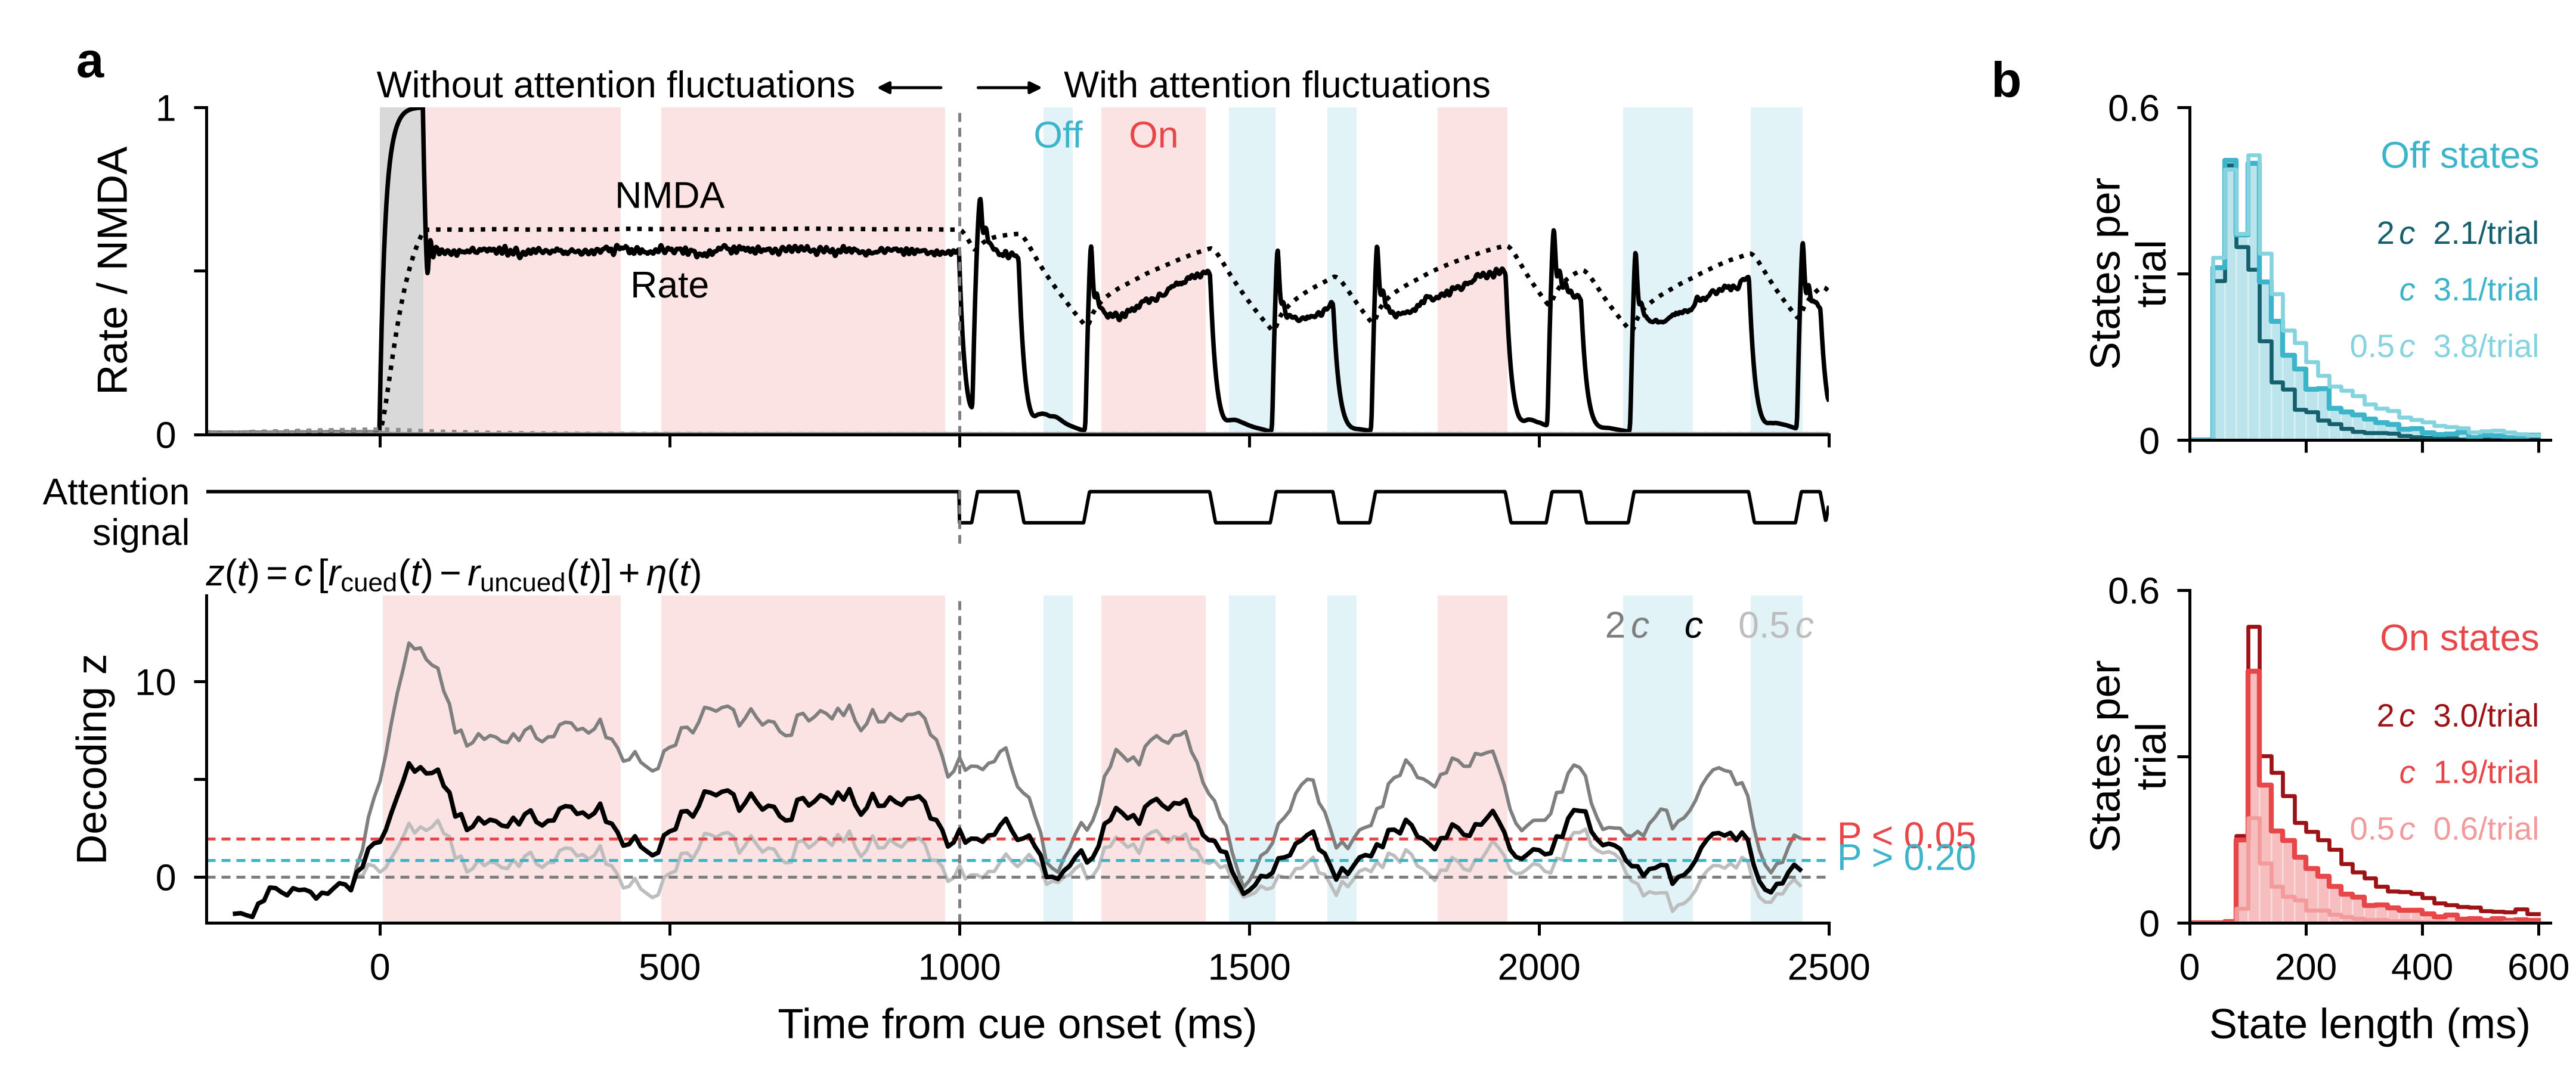
\includegraphics[width=\textwidth]{fig1_trial_histograms.png}
  \caption{\textbf{Input dips create On and Off states, and NMDA carries the memory.} \textbf{a}, Example trial. Top: rates of the cued (black) and uncued (grey) pools, relative to the maximum rate, and their NMDA gating (dotted); grey shading marks the cue. Middle: common input (attention signal), constant for the first 1,000~ms after the cue and with dips afterwards. The dip-free first second is shown for illustration only; in all other simulated trials, dips occur throughout the delay. Bottom: decoding $z$ score, with On (red) and Off (cyan) states. Dashed lines: On threshold ($z = 1.96$) and Off threshold ($z = 0.84$), as in \citet{panichello2024}. \textbf{b}, Length distributions of Off (top) and On (bottom) states in the model.}
  \label{fig:1}
\end{figure}

\subsection{On/Off statistics depend on which neurons are decoded}

So far we considered decoders that use all recorded neurons. We found, however, that On/Off statistics depend strongly on which neurons the decoder uses, which we call the decoded population (Fig.~2, black circles). Decoders using the most cue-selective neurons spend much more of the delay On, and less Off, than decoders using the same numbers of randomly chosen neurons, which also show more Off states per trial. The decoded populations differ mainly in decoding strength, which is much higher for the most selective neurons. How often a memory appears Off therefore depends partly on how well the recorded neurons read it out. This matters for interpreting Off states as evidence for activity-silent memory: a decoder trained on a limited sample of neurons can fall to chance while the memory is still present in the activity of other, unrecorded neurons. The measured fraction of Off states is therefore an upper bound on, not a measure of, how often the memory leaves spiking activity.

\begin{figure}[t]
  \centering
  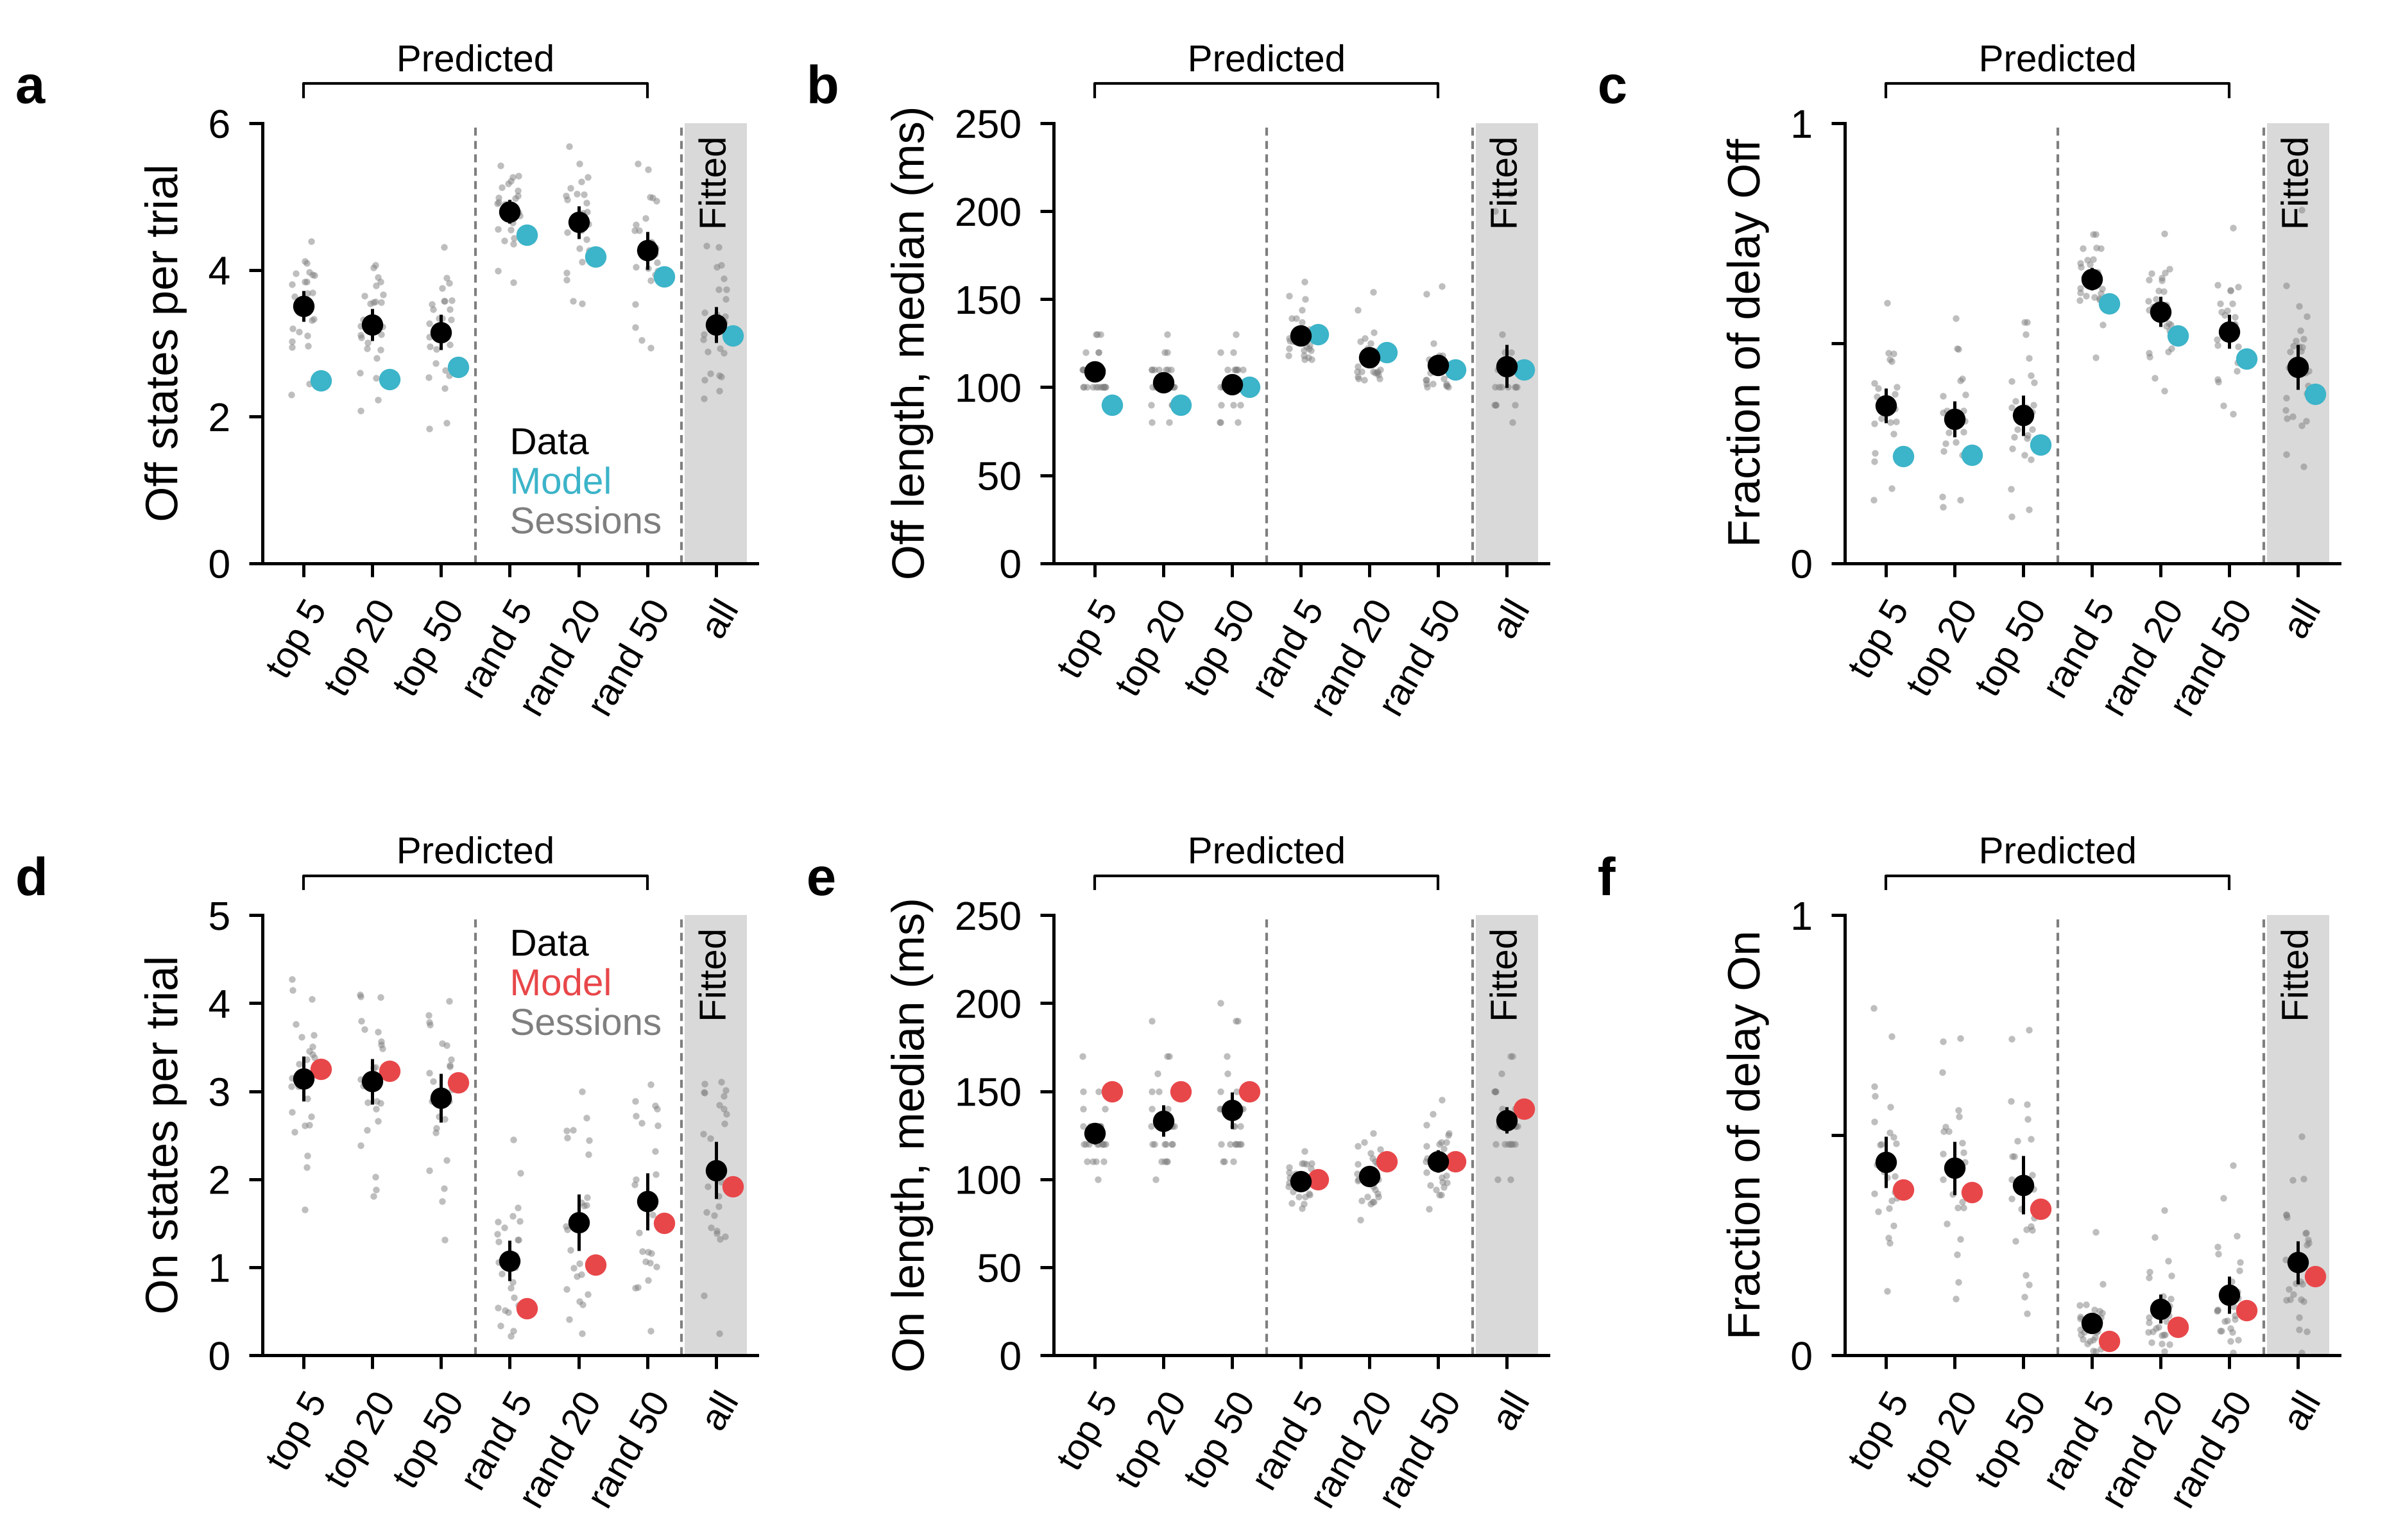
\includegraphics[width=0.92\textwidth]{fig2_unit_sets.png}
  \caption{\textbf{The model predicts how On/Off statistics change with the decoded population.} Decoders using the most cue-selective neurons (top 5, 20, 50) are On more often and Off less often than decoders using the same numbers of random neurons (rand 5, 20, 50). Black circles: data, mean $\pm$ 95\% CI (2 SEM) over 25 sessions. Grey dots: single sessions. Cyan and red circles: model, Off and On statistics. The model was fitted to all neurons only (grey bar); the other six decoded populations are predictions obtained by changing only the read-out gain and noise.}
  \label{fig:2}
\end{figure}

\subsection{A model fitted to all neurons predicts this dependence}

Can our model explain this dependence? If Off states come from shared dips in network activity, the same dynamics, read out with a higher or lower decoding strength, should reproduce the change across decoded populations. To test this, we fitted seven parameters of the dynamics only to the decoder using all neurons in 25 sessions (Methods). The model matches the data in Off states per trial (3.1 vs 3.3), Off median length (110 vs 112~ms), On states per trial (1.9 vs 2.1) and On median length (140 vs 134~ms) (Fig.~2, grey band). We then kept the dynamics fixed and, for each of the six other decoded populations, changed only the read-out without fitting any parameters: its gain was calibrated on that population's decoding strength, and its noise on that population's pre-cue $z$ (Methods). Without any refitting, the model predicts quantitatively the shift between selective and random neurons.

\section{Discussion}

Recent large-scale recordings agree that prefrontal decoding of a remembered item is intermittent on single trials, but differ on whether Off states mean that the memory leaves spiking activity and is held in short-term synaptic plasticity \citep{panichello2024,tao2024,mozumder2026}. We showed that the same On/Off statistics arise in a conventional attractor network with fixed synapses. Off states occur when a common input briefly drops, and the memory survives each silence because NMDA receptor currents decay slowly enough to bias which pool restarts. Fitted to the decoder trained on the empirical data, the model reproduced the number and length of On and Off states and kept the memory in 98\% of trials.

In the recordings, Off states were more frequent and On states rarer when the decoder used random rather than selective neurons. This showed that a decoder falls to chance whenever the memory signal in its sample is weak relative to its noise, not only when the memory is absent from the network. The fraction of time Off measured from a limited sample is therefore an upper bound on how often the memory leaves spiking activity, and comparisons of Off-state statistics across studies or brain areas need to take the decoded population into account. The model captured this shift without refitting by changing only the read-out gain and noise, both calibrated from the data.

Our account is consistent with the other recent recordings of Off states. \citet{mozumder2026} found that Off states were synchronized between prefrontal and posterior parietal cortex, came with lower firing rates, and showed no obvious rhythmicity. A common input that reaches several areas and fluctuates irregularly, as in our fit, would produce such coordinated, aperiodic Off states. They also found that tuning was reduced by about 78\% but not abolished during Off states, in line with our finding that Off states depend on how well the decoded population reads out the memory; in our model, a shallower dip that weakens rather than silences the memory pool would have the same effect. \citet{tao2024} likewise found that information is reduced but present between gamma bursts. Their rare silences of all selective neurons, lasting up to 414~ms, are the strongest evidence for activity-silent storage. NMDA currents can bridge silences of about 100~ms in our model, but the longest of these events exceed that time scale and may require slower mechanisms.

We interpreted the common input as an attentional signal that is high when attention is deployed on the memorandum and drops during lapses. This links intermittent decoding to evidence that sustained attention samples rhythmically rather than continuously. In humans, detection of threshold stimuli depends on the phase of ongoing EEG oscillations near 7~Hz \citep{busch2009}, but only at attended locations \citep{busch2010}. When attention is divided between two locations, detection at each fluctuates at about 4~Hz, in antiphase between locations \citep{landau2012}, and sampling occurs at about 8~Hz within an attended object and at about 4~Hz between objects \citep{fiebelkorn2013}. In monkeys, frontal eye field and lateral intraparietal activity alternates at theta frequencies (3–8~Hz) between periods of enhanced perception and periods in which attention is more likely to shift \citep{fiebelkorn2018}, and human intracranial recordings show similar theta-rhythmic sampling in frontoparietal cortex \citep{helfrich2018}. These findings have been unified in a rhythmic theory of attention, in which theta rhythms alternate between sampling and shifting \citep{fiebelkorn2019}. Because attention and working memory share prefrontal mechanisms \citep{awh2001,panichello2021}, lapses of attention could plausibly reach the memory network. In the fitted model, the attention signal recovers about five times per second, one cycle every ${\sim}$200~ms. This is in the low theta range reported for attentional sampling \citep{landau2012,fiebelkorn2018,helfrich2018} and slower than the ${\sim}$7~Hz phase effects on detection \citep{busch2009,busch2010}. Attention episodes lasted 72~ms (median) and lapses 88~ms, so attention was deployed about half of the time. However, the fitted signal was not periodic. Consistent with this, intervals between successive Off-state onsets were irregular in both the model (coefficient of variation 0.59) and the recordings (0.62), although interval regularity was not part of the fit. The data therefore favour a quasi-rhythmic or irregular sampling process over a strict pacemaker. A direct test would be to ask whether Off-state onsets lock to the phase of theta activity in the prefrontal local field potential, or whether probes presented during Off states are detected less often.

In our model, the memory is carried across each silence by NMDA gating. This is a synaptic variable, but it decays within ${\sim}$150~ms and reflects recent firing rather than plasticity. Off states last about 100~ms, within the time an NMDA trace can bridge, so no longer-lasting mechanism is needed to explain them. Activity-silent mechanisms may still matter on longer time scales, for example to carry information between trials, when prefrontal memory traces are reactivated before the next stimulus \citep{barbosa2020}. Persistent activity and slower silent traces are therefore not mutually exclusive; our results only show that intermittent decoding within a delay does not require the latter.

\paragraph{Limitations.} First, the model restarts the memory with a brief transient: when the common input returns, excitation precedes lagging feed-forward inhibition by ${\sim}$15~ms. Without such a transient, pools silenced by a dip often failed to restart. We implemented it as feed-forward inhibition, a common circuit motif, but recovery of input synapses from depression during a dip would produce a similar onset overshoot. Second, two fitted parameters ended at the bounds of the search: the NMDA decay time ($\tau_{N}$ = 150~ms, upper bound) and the recurrent NMDA strength ($w_{s}$, lower bound), so the model needs the slowest NMDA currents we considered plausible. Third, the model spent slightly less of the delay in both On and Off states than the data, underestimated the number of Off states for the most selective neurons, and predicted too few On states for small random populations. A single linear read-out of two pools may be too simple for decoders based on a few noisy neurons. Fourth, the common input silences both memory pools together, whereas attention modulates detection only at attended locations \citep{busch2010}. An attentional input acting selectively on the populations that carry the memory, rather than as a global silence, remains to be tested.

Intermittent decoding of working memory is expected from an attractor network with slow NMDA currents and a fluctuating, attention-like input, and its statistics depend on how well the recorded neurons read out the memory. These results reconcile intermittent rate coding with persistent-activity accounts and link Off states to the rhythmic, irregular nature of attentional sampling.

\section{Methods}

\subsection{Rate model}

Two excitatory memory pools $X \in \{\cued, \uncued\}$ have rates $r_X$ and NMDA gating $s_X$.
They share an inhibitory population $r_I$ and a feed-forward inhibition $q$ that follows the common input $m(t)$ with a lag:
\begin{align}
  \tau_r \frac{dr_X}{dt} &= -r_X + \Phi\bigl(w_s s_X + w_a r_X - w_I r_I + I_0\, m(t) - w_{\mathit{ff}}\, q + \mathrm{cue}_X + \sigma \xi_X\bigr), \\
  \tau_N \frac{ds_X}{dt} &= -s_X + \beta\, r_X (1 - s_X), \\
  \tau_I \frac{dr_I}{dt} &= -r_I + w_{EI} \left(r_\cued + r_\uncued\right), \\
  \tau_{\mathit{ff}} \frac{dq}{dt} &= -q + m(t).
\end{align}
$\Phi(x) = r_{\max} / \bigl(1 + \exp(-(x - 1)/\kappa)\bigr)$, and $\xi_X$ are independent Ornstein--Uhlenbeck noises ($\tau_\xi = 10$~ms).
Fixed parameters: $r_{\max} = 150$, $\kappa = 0.06$, $w_a = 0.0141$, $\beta = 0.02$, $w_I = 0.04$, $w_{EI} = 0.5$, $w_{\mathit{ff}} = 0.8$, $I_0 = 1.496$; $\tau_r = 10$~ms, $\tau_I = 1$~ms, $\tau_{\mathit{ff}} = 15$~ms.
The cue is a 50~ms input of amplitude 1 to the cued pool, after 300~ms of baseline, followed by a 1,600~ms delay.
Equations were integrated with Euler steps of 0.1~ms.
The memory was scored correct when, in the last 100~ms, the NMDA gating of the cued pool exceeded the uncued pool's by more than 0.05.

The common input $m(t)$ is 1 except during dips, where it drops to $1 - \delta$ with 10~ms ramps.
Dip lengths are gamma-distributed (mean $\mu_d$, shape $k$), and the gaps between dips are exponential with mean $1/\lambda_d$.

\subsection{Decoding read-out, On/Off labelling and statistics}

The decoder $z$ score was modelled as $z(t) = c\, \Delta r(t) + \eta(t)$, where $\Delta r$ is the cued minus uncued rate in 100~ms windows stepped by 10~ms.
The noise $\eta$ has unit variance, the autocorrelation of overlapping windows, and a slow per-trial offset whose variance share was measured from the pre-cue $z$ of the data (0.35 for all neurons, 0.09 for the most selective neurons, 0.11 for random neurons).
The gain $c$ was not fitted: for each decoded population, it was chosen so that the upper mean of a two-component Gaussian mixture of delay $z$ values matched the data's.
We call this upper mean the decoding strength.
States were labelled as in \citet{panichello2024}.
On states are runs of $z > 1.96$ whose summed $z$ exceeds the 95th percentile of the same quantity in pure noise.
Off states are runs of at least 5 points (50~ms) with $z < 0.84$.
States were counted from 0 to 1,400~ms after cue onset, and fractions of the delay spent On or Off from 500 to 1,400~ms.
Model statistics were computed from 2,112 simulated trials (792 per evaluation during fitting).
Data statistics are means over the 25 sessions; for random neurons, the 10 draws were first averaged within each session.

\subsection{Data}

We reanalysed the recordings of \citet{panichello2024}: 25 sessions, correct trials only, all cue locations (13,190 trials; 329 units per session on average).
For each time bin, an L2-regularised logistic decoder ($\lambda = 10{,}000$) was evaluated with approximate leave-one-out and $z$-scored against 30 shuffled label sets per cue pair.
Decoded populations were all neurons, the $k$ most cue-selective neurons (ranked by split-half ANOVA), and $k$ randomly chosen neurons (10 draws, averaged within sessions), with $k = 5$, 20 and 50.

\subsection{Fitting}

Seven parameters were fitted with CMA-ES to the decoder using all neurons only: $\tau_N$, $w_s$, $\lambda_d$, $\mu_d$, $k$, $\delta$ and $\sigma$.
The loss combined the squared scaled errors of six statistics (On and Off states per trial, mean lengths and fractions of the delay), the squared Hellinger distance between model and data length distributions (states $\geq 40$~ms), and a penalty when the memory was correct in fewer than 98\% of trials.
Best fit: $\tau_N = 150$~ms, $w_s = 1.30$, $\lambda_d = 10.2$/s, $\mu_d = 90$~ms, $k = 8.7$, $\delta = 0.60$, $\sigma = 0.006$.
$\tau_N$ and $w_s$ ended at the bounds of the search (50--150~ms and 1.30--1.70).

Code: \texttt{paper\_model/} on the \texttt{paper-model} branch of the \texttt{gamma\_bursts-} repository.

\bibliographystyle{plainnat}
\bibliography{refs}

\end{document}
